\documentclass[12pt,openright,twoside,a4paper,english,french,spanish,brazil]{abntex2}

\usepackage{cmap}	
\usepackage{lmodern}	
\usepackage[T1]{fontenc}	
\usepackage[utf8]{inputenc}		
\usepackage{lastpage}		
\usepackage{indentfirst}
\usepackage{color}
\usepackage{graphicx}
\usepackage{units}
\usepackage[brazilian,hyperpageref]{backref}
\usepackage[alf]{abntex2cite}
\usepackage{bold-extra}
\usepackage{eso-pic}
\usepackage{multirow}
\usepackage{url}
\usepackage{float}
\usepackage[table,xcdraw]{xcolor}
\usepackage{listings}
\usepackage{threeparttable}
\usepackage{float}
\floatstyle{plaintop} % Coloca caption no topo
\newfloat{quadro}{htbp}{lop}
\floatname{quadro}{Quadro}
\newcommand{\listofquadros}{\listof{quadro}{Lista de Quadros}}

\renewcommand{\backrefpagesname}{Citado na(s) página(s):~}
\renewcommand{\backref}{}
\renewcommand*{\backrefalt}[4]{
	\ifcase #1 %
		Nenhuma citação no texto.%
	\or
		Citado na página #2.%
	\else
		Citado #1 vezes nas páginas #2.%
	\fi}%
% ---


\usepackage{fixos/customizacoes}

% Dados pessoais
\autor{Gustavo Marques Lima}
\curso{Engenharia de Software}

% Dados do trabalho
\titulo{Título: Projeto do Gamma Online Judge}
\data{2021}
\palavraChaveUm{projeto}
\palavraChaveDois{Online Judge}

% Dados da orientacao
\orientador{Titulação Acadêmica e Nome do Orientador}
\coorientador{quando houver, Titulação Acadêmica e Nome do Orientador}

% Dados para a ficha catalográfica
\cdu{02:141:005.6}

% Dados da aprovação do trabalho
\dataDaAprovacao{01 de junho de 2013 -- Data da aprovação do trabalho}
\membroConvidadoUm{Titulação e Nome do Professor Convidado 01}
\membroConvidadoDois{Titulação e Nome do Professor Convidado 02}

% Dados pessoais
\autor{Gustavo Marques Lima}
\curso{Engenharia de Software}

% Dados do trabalho
\titulo{Título: Projeto do Gamma Online Judge}
\data{2021}
\palavraChaveUm{projeto}
\palavraChaveDois{Online Judge}

% Dados da orientacao
\orientador{Titulação Acadêmica e Nome do Orientador}
\coorientador{quando houver, Titulação Acadêmica e Nome do Orientador}

% Dados para a ficha catalográfica
\cdu{02:141:005.6}

% Dados da aprovação do trabalho
\dataDaAprovacao{01 de junho de 2013 -- Data da aprovação do trabalho}
\membroConvidadoUm{Titulação e Nome do Professor Convidado 01}
\membroConvidadoDois{Titulação e Nome do Professor Convidado 02}

\definecolor{blue}{RGB}{41,5,195}
\makeatletter
\hypersetup{
     	%pagebackref=true,
		pdftitle={\@title}, 
		pdfauthor={\@author},
    	pdfsubject={\imprimirpreambulo},
	    pdfcreator={LaTeX with abnTeX2},
		pdfkeywords={abnt}{latex}{abntex}{abntex2}{trabalho acadêmico}, 
		colorlinks=true,       		% false: boxed links; true: colored links
    	linkcolor=blue,          	% color of internal links
    	citecolor=blue,        		% color of links to bibliography
    	filecolor=magenta,      		% color of file links
		urlcolor=blue,
		bookmarksdepth=4
}
\makeatother
\setlength{\parindent}{1.3cm}
\setlength{\parskip}{0.2cm}  
\makeindex


\begin{document}

\frenchspacing
\imprimircapa
\imprimirfolhaderosto*

\begin{fichacatalografica}
	\vspace*{\fill}					% Posição vertical
	\hrule							% Linha horizontal
	\begin{center}					% Minipage Centralizado
	\begin{minipage}[c]{12.5cm}		% Largura
	
	\imprimirautor
	
	\hspace{0.5cm} \imprimirtitulo  / \imprimirautor. --
	\imprimirlocal, \imprimirdata-
	
	\hspace{0.5cm} \pageref{LastPage} p. : il. (algumas color.) ; 30 cm.\\
	
	\hspace{0.5cm} \imprimirorientadorRotulo~\imprimirorientador\\
	
	\hspace{0.5cm}
	\parbox[t]{\textwidth}{\imprimirtipotrabalho~--~\imprimirinstituicao,
	\imprimirdata.}\\
	
	\hspace{0.5cm}
		1. \imprimirpalavrachaveum.
		2. \imprimirpalavrachavedois.
		I. \imprimirorientador.
		II. Universidade de Brasília.
		III. Faculdade UnB Gama.
		IV. \imprimirtitulo\\ 			
	
	\hspace{8.75cm} CDU \nomecdu\\
	
	\end{minipage}
	\end{center}
	\hrule
\end{fichacatalografica}

\input{editaveis/errata}
\begin{folhadeaprovacao}

  \begin{center}
    {\ABNTEXchapterfont\large\imprimirautor}

    \vspace*{\fill}\vspace*{\fill}
    {\ABNTEXchapterfont\bfseries\Large\imprimirtitulo}
    \vspace*{\fill}
    
    \hspace{.45\textwidth}
    \begin{minipage}{.5\textwidth}
        \imprimirpreambulo
    \end{minipage}%
    \vspace*{\fill}
   \end{center}
    
   Trabalho aprovado. \imprimirlocal, \imprimirdatadaaprovacao:

   \assinatura{\textbf{\imprimirorientador} \\ Orientador} 
   \assinatura{\textbf{\imprimirmembroconvidadoum} \\ Convidado 1}
   \assinatura{\textbf{\imprimirmembroconvidadodois} \\ Convidado 2}
      
   \begin{center}
    \vspace*{0.5cm}
    {\large\imprimirlocal}
    \par
    {\large\imprimirdata}
    \vspace*{1cm}
  \end{center}
  
\end{folhadeaprovacao}

\begin{dedicatoria}
   \vspace*{\fill}
   \centering
   \noindent

   \textit{Este trabalho é dedicado aos novos estudantes de programação competitiva do gama.} \vspace*{\fill}

\end{dedicatoria}

\begin{agradecimentos}

    Agradeço as pessoas que me apoiaram e me motivaram durante a escrita desse texto, agradeço ao meu professor Edson que sempre me motivou a seguir como programador competitivo, agradeço a minha família que me deu apoio durante todo o meu curso e agradeço a minha namorada que sempre esteve comigo a todo momento, me apoiando e me ajudando.

\end{agradecimentos}

\begin{epigrafe}
	\vspace*{\fill}
	\begin{flushright}

		\textit{``Já fui jovem e agora sou velho, \\
			mas nunca vi o justo desamparado \\
			anem seus filhos mendigando o pão \\
			(Bíblia Sagrada, Salmos 37, 25)}
	\end{flushright}
\end{epigrafe}

\begin{resumo}

    O trabalho consistem em um projeto desenvolvido em NodeJS, React e Typescript
    para a construção de um juíz online contendo questões das maratonas de programação UnB,
    realizadas em várias edições diferentes. O projeto consiste na criação de um site contendo 
    as questões das maratonas de programação realizadas, e possibilita que competidores tenham 
    acesso as questões e submetam suas soluções para os problemas, com um feedback rápido.

 \vspace{\onelineskip}
    
 \noindent
 \textbf{Palavras-chave}: online judge. projeto. react. node. typescript.
\end{resumo}

\begin{resumo}[Abstract]
 \begin{otherlanguage*}{english}
 
   The Gamma Online Judge is an online judge, containing questions from Maratonas UnB de Programação. It aims to bring together the questions from past events editions on a platform, enabling users to test their solutions to the event's problems. Gamma Online Judge is a project, and it is being developed with Node and React, using Typescript as the main language. The system is divided into microservices with individual responsibilities.

   \vspace{\onelineskip}
 
   \noindent 
   \textbf{Key-words}: online judge. project. react. node. typescript. programming contests. gamma online judge.
   
 \end{otherlanguage*}
\end{resumo}

\pdfbookmark[0]{\listfigurename}{lof}
\listoffigures*
\cleardoublepage
\pdfbookmark[0]{\listtablename}{lot}
\listoftables*
\listofquadros
\cleardoublepage

\begin{siglas}
  \item[HTML] HyperText Markup Language
  \item[TLE] Time Limit Exceeded
  \item[MLE] Memory Limit Exceeded
  \item[WA] Wrong Answer 
  \item[vX.X.X] Versão X.X.X
\end{siglas}

\input{editaveis/simbolos}
\pdfbookmark[0]{\contentsname}{toc}
\tableofcontents*
\cleardoublepage


\textual

part{Introdução}

\chapter[Introdução]{Introdução}

\section{Contextualização}

O trabalho consiste em um juiz online para armazenar e julgar códigos de questões das edições da maratonas UnB de programação. 
Durante os anos foram realizadas várias edições das maratonas de programação UnB, que são eventos para competidores testar e aprimorar as suas habilidades de programação e resolução de problemas. Em geral essas maratonas são interessantes para alunos iniciantes e intermediários em programação competitiva, pois os problemas variam entre problemas fáceis e mais difíceis. Essas maratonas foram realizadas internamente, muitas vezes sem auxílio de ferramentas externas e servidores externos, o que dificulta os competidores a encontrar questões antigas de edições passadas, encontrar resolução e tutoriais para as questões, e o mais importante, uma plataforma para testar seus códigos, processo que é fundamental para aprendizagem na área. 
Existem vários juízes online que fazem esse trabalho de armazenar e julgar questões, os mais populares no meio da programação para competição no Brasil são o Online Judge, URI e o Codeforces, porém o processo para criar eventos e centralizar as questões nesses juízes não é ideal. Dentre eles só o URI é disponibilizado em português, nele um usuário comum não consegue criar questões originais, e mesmo criando questões os tutoriais e dicas não são feitos da maneira ideal, as ferramentas proporcionadas são um uDebug e um fórum para discussão, que ajudam, porém não é ideal, pois o feedback de um fórum não é imediato, o que pode desencorajar estudantes a procurarem essa plataforma para esse tipo de uso. O Codeforces é um ótimo juíz e bastante conhecido por ser uma plataforma mais aberta, nele é possível ver o código de outros competidores em competições oficiais, após a competição, e nos principais eventos são disponibilizados tutoriais para as questões, para auxiliar o competidor que teve muita dificuldade e tem curiosidade de saber como é a resolução de uma questão específica, o que impede a utilização dessa plataforma é que a linguagem oficial do site é inglês e não é possível criar questões e eventos no site, apenas em grupos, o que dificulta a catalogação e indexação dos problemas.
O projeto consiste em um repositório que armazenará as questões das edições anteriores das maratonas de programação, separando as questões por edição das maratonas de programação e facilitando a busca de questões antigas. O sistema também disponibilizará tags que separam as questões por tópicos, o que é interessante para treinamento de um tópico específico. A plataforma disponibilizará os enunciados, dicas e tutoriais de como resolver os problemas e um juíz online que julgará as soluções dos competidores interessados em treinar suas soluções para essas questões de edições passadas, com isso o feedback para a resolução dos problemas e busca de soluções será imediato, o que motiva mais o competidor.


\section{Justificativa/Motivação}

O primeiro contato que eu tive com um juíz online foi no primeiro semestre da faculdade na disciplina de Algoritmos e Programação para Computadores, nessa disciplina era ensinado programação básica, e o meu professor utilizava o juíz online URI. Nele o feedback para resolução dos problemas era imediato, eu sabia quando um código estava errado, lento ou inadequado para aquele problema, o que facilitava mais no aprendizado pois eu não dependia de um professor corrigir meu código para saber se estava certo. No terceiro semestre da faculdade tive um contato maior com esse tipo de Juíz online pois entrei no mundo de programação competitiva, eu competi em várias edições da Maratona UnB de programação, o que me motivou a participar da seletiva de programação, que me rendeu uma vaga para competir na Final brasileira de programação em campina grande, lá eu obtive o 26º lugar do brasil em programação. Dentre todas as maratonas que eu fiz eu percebi que o armazenamento desses eventos geralmente não é feito de forma ideal, com exceção de alguns eventos como competições da Olimpíada Brasileira de Informática, que tem um site próprio para armazenar questões de edições passadas, eventos próprios de plataformas, como os contests do Codeforces, porém muitos eventos não possuem uma plataforma que disponibiliza os enunciados e tutoriais dessas questões e julgam solução para auxiliar competidores a treinar e aprender mais. Fiz várias das maratonas UnB de programação e em geral as questões desses eventos são muito boas para iniciantes aprenderem sobre tópicos clássicos de programação competitiva, acredito que uma plataforma para o armazenamento dessas questões será uma ótima ferramenta para novos competidores estudarem.
O trabalho a princípio será desenvolvido por mim e futuramente mantido por outras pessoas, visto isso, a tecnologia utilizada foi Node JS, tanto na interface quanto no servidor para facilitar a contextualização de contribuidores, e o aprendizado de interessados em contribuir com o projeto, sendo que na interface é utilizado o React como framework para criação das telas. A linguagem de programação utilizada tanto na interface, quanto no servidor foi Typescript pelo fato de ser uma linguagem de programação fortemente tipada, não foi optado a utilização de Javascript, que é uma linguagem mais comum para a tecnologia, pois apesar do ganho de tempo ao se preocupar menos com a tipagem, erros futuros podem ser mais difíceis de se encontrar erros no código e revisar códigos de contribuidores pode ser mais complicado, com uma linguagem fortemente tipada boa parte do processo de análise é feito pelo compilador, e com um editor de texto configurado erros ficam mais visuais. O servidor se comunica com um banco de dados orientado a documento, o MongoDB, pois nesse projeto a flexibilidade do banco em relação ao armazenamento de documento é mais interessante que um banco de dados relacional. A popularidade entre Node e MongoDB foi outro fator para a escolha dessa tecnologia. 
	

\section{Objetivos}

\subsection{Objetivo Geral} 

Criar plataforma para armazenar e julgar questões das edições anteriores das Maratonas UnB de programação

\subsection{Objetivos específicos}

Criação de banco de dados para armazenar questões e eventos das maratonas UnB de programação e as submissões dos usuários 
Criação de uma interface que possibilita um usuário encontrar, buscar, ler e enviar questões
Criação de um micro serviço para criar, editar, deletar e fazer busca em questões e eventos. Esse serviço será utilizado pela interface.
Criação  de um micro serviço para receber códigos dos usuários, julgá-los e retornar o veredito. Esse serviço será utilizado pela interface.

\section{Estrutura do Trabalho}

-


part{Fundamentação Teórica}

\chapter[Fundamentação Teórica]{Fundamentação Teórica}

Estas instruções apresentam um conjunto mínimo de exigências necessárias a 
uniformidade de apresentação do relatório de Trabalho de Conclusão de Curso 
da FGA. Estilo, concisão e clareza ficam inteiramente sob a 
responsabilidade do(s) aluno(s) autor(es) do relatório.

As disciplinas de Trabalho de Conclusão de Curso (TCC) 01 e Trabalho de 
Conclusão de Curso (TCC) 02 se desenvolvem de acordo com Regulamento 
próprio aprovado pelo Colegiado da FGA. Os alunos matriculados nessas 
disciplinas devem estar plenamente cientes de tal Regulamento. 

\section{Composição e estrutura do trabalho}

A formatação do trabalho como um todo considera três elementos principais: 
(1) pré-textuais, (2) textuais e (3) pós-textuais. Cada um destes, pode se 
subdividir em outros elementos formando a estrutura global do trabalho, 
conforme abaixo (as entradas itálico são \textit{opcionais}; em itálico e
negrito são \textbf{\textit{essenciais}}):

\begin{description}
	\item [Pré-textuais] \

	\begin{itemize}
		\item Capa
		\item Folha de rosto
		\item \textit{Dedicatória}
		\item \textit{Agradecimentos}
		\item \textit{Epígrafe}
		\item Resumo
		\item Abstract
		\item Lista de figuras
		\item Lista de tabelas
		\item Lista de símbolos e
		\item Sumário
	\end{itemize}

	\item [Textuais] \

	\begin{itemize}
		\item \textbf{\textit{Introdução}}
		\item \textbf{\textit{Desenvolvimento}}
		\item \textbf{\textit{Conclusões}}
	\end{itemize}

	\item [Pós-Textuais] \
	
	\begin{itemize}
		\item Referências bibliográficas
		\item \textit{Bibliografia}
		\item Anexos
		\item Contracapa
	\end{itemize}
\end{description}

Os aspectos específicos da formatação de cada uma dessas três partes 
principais do relatório são tratados nos capítulos e seções seguintes.

No modelo \LaTeX, os arquivos correspondentes a estas estruturas que devem
ser editados manualmente estão na pasta \textbf{editáveis}. Os arquivos
da pasta \textbf{fixos} tratam os elementos que não necessitam de 
edição direta, e devem ser deixados como estão na grande maioria dos casos.

\section{Considerações sobre formatação básica do relatório}

A seguir são apresentadas as orientações básicas sobre a formatação do
documento. O modelo \LaTeX\ \textbf{já configura todas estas opções corretamente},
de modo que para os usuários deste modelo o texto de toda esta Seção é 
\textbf{meramente informativo}.

\subsection{Tipo de papel, fonte e margens}

Papel -- Na confecção do relatório deverá ser empregado papel branco no 
formato padrão A4 (21 cm x 29,7cm), com 75 a 90 g/m2.

Fonte -- Deve-se utilizar as fontes Arial ou Times New Roman no tamanho 12 
pra corpo do texto, com variações para tamanho 10 permitidas para a 
wpaginação, legendas e notas de rodapé. Em citações diretas de mais de três 
linhas utilizar a fonte tamanho 10, sem itálicos, negritos ou aspas. Os 
tipos itálicos são usados para nomes científicos e expressões estrangeiras, 
exceto expressões latinas.

Margens -- As margens delimitando a região na qual todo o texto deverá estar 
contido serão as seguintes: 

\begin{itemize}
	\item Esquerda: 03 cm;
	\item Direita	: 02 cm;
	\item Superior: 03 cm;
	\item Inferior: 02 cm. 
\end{itemize}

\subsection{Numeração de Páginas}

A contagem sequencial para a numeração de páginas começa a partir da 
primeira folha do trabalho que é a Folha de Rosto, contudo a numeração em 
si só deve ser iniciada a partir da primeira folha dos elementos textuais. 
Assim, as páginas dos elementos pré-textuais contam, mas não são numeradas 
e os números de página aparecem a partir da primeira folha dos elementos 
textuais, que se iniciam na Introdução. 

Os números devem estar em algarismos arábicos (fonte Times ou Arial 10) no 
canto superior direito da folha, a 02 cm da borda superior, sem traços, 
pontos ou parênteses. 

A paginação de Apêndices e Anexos deve ser contínua, dando seguimento ao 
texto principal.

\subsection{Espaços e alinhamento}

Para a monografia de TCC 01 e 02 o espaço entrelinhas do corpo do texto 
deve ser de 1,5 cm, exceto RESUMO, CITAÇÔES de mais de três linhas, NOTAS 
de rodapé, LEGENDAS e REFERÊNCIAS que devem possuir espaçamento simples. 
Ainda, ao se iniciar a primeira linha de cada novo parágrafo se deve 
tabular a distância de 1,25 cm da margem esquerda.

Quanto aos títulos das seções primárias da monografia, estes devem começar 
na parte superior da folha e separados do texto que o sucede, por um espaço 
de 1,5 cm entrelinhas, assim como os títulos das seções secundárias, 
terciárias. 

A formatação de alinhamento deve ser justificado, de modo que o texto fique 
alinhado uniformemente ao longo das margens esquerda e direita, exceto para 
CITAÇÕES de mais de três linhas que devem ser alinhadas a 04 cm da margem 
esquerda e REFERÊNCIAS que são alinhadas somente à margem esquerda do texto 
diferenciando cada referência.

\subsection{Quebra de Capítulos e Aproveitamento de Páginas}

Cada seção ou capítulo deverá começar numa nova pagina (recomenda-se que 
para texto muito longos o autor divida seu documento em mais de um arquivo 
eletrônico). 

Caso a última pagina de um capitulo tenha apenas um número reduzido de 
linhas (digamos 2 ou 3), verificar a possibilidade de modificar o texto 
(sem prejuízo do conteúdo e obedecendo as normas aqui colocadas) para 
evitar a ocorrência de uma página pouco aproveitada.

Ainda com respeito ao preenchimento das páginas, este deve ser otimizado, 
evitando-se espaços vazios desnecessários. 

Caso as dimensões de uma figura ou tabela impeçam que a mesma seja 
posicionada ao final de uma página, o deslocamento para a página seguinte 
não deve acarretar um vazio na pagina anterior. Para evitar tal ocorrência, 
deve-se reposicionar os blocos de texto para o preenchimento de vazios. 

Tabelas e figuras devem, sempre que possível, utilizar o espaço disponível 
da página evitando-se a \lq\lq quebra\rq\rq\ da figura ou tabela. 

\section{Cópias}

Nas versões do relatório para revisão da Banca Examinadora em TCC1 e TCC2, 
o aluno deve apresentar na Secretaria da FGA, uma cópia para cada membro da 
Banca Examinadora.

Após a aprovação em TCC2, o aluno deverá obrigatoriamente apresentar a 
versão final de seu trabalho à Secretaria da FGA na seguinte forma:

\begin{itemize}
	\item 01 cópia encadernada para arquivo na FGA;
	\item 01 cópia não encadernada (folhas avulsas) para arquivo na FGA;
	\item 01 cópia em CD de todos os arquivos empregados no trabalho.
\end{itemize}

A cópia em CD deve conter, além do texto, todos os arquivos dos quais se 
originaram os gráficos (excel, etc.) e figuras (jpg, bmp, gif, etc.) 
contidos no trabalho. Caso o trabalho tenha gerado códigos fontes e 
arquivos para aplicações especificas (programas em Fortran, C, Matlab, 
etc.) estes deverão também ser gravados em CD. 

O autor deverá certificar a não ocorrência de “vírus” no CD entregue a 
secretaria. 


\chapter[Metodologia]{Metodologia}

\section{Metodologia de desenvolvimento}

O desenvolvimento da aplicação foi feito de maneira individual, e para organização do desenvolvimento foi feito primeiro um levantamento de requisitos. Os requisitos da aplicação foram esses:
\begin{enumerate}

    \item É necessário armazenar um número limitado de questões e eventos das maratonas UnB com atualização não frequente
    \item O visitante do site deve ter capacidade de enviar sua solução em código para que ela seja julgada, e em pouco tempo ele deve receber o veredicto de sua submissão, caso passe em todos os testes o sistema deve deixar claro que seu código foi aceito, caso contrário o sistema deve apresentar uma mensagem exemplificando o erro como TLE, MLE, RE.
    \item O visitante do site deve conseguir ter acesso aos problemas e eventos por um site, a tutoriais e dicas das questões, sendo que as dicas sejam frases que auxiliam o visitante na resolução do problema e o tutorial um guia completo sobre uma abordagem de solução do problema
\end{enumerate}

Dentro desses requisitos básicos as tarefas foram separadas em épicos e quebradas em tarefas menores, dentre todas as tarefas menores o nível de priorização foi feita com base em meu conhecimento em tecnologias, os requisitos que eu tinha conhecimento que poderiam ser cumpridos tiveram uma prioridade menor, pois caso algum requisito fosse mais difĩcil ou exigisse mais tempo de estudo para ser cumprido eu poderia avaliar alternativas.

Os requisitos citados acima estão feitos de uma maneira mais ampla e precisam ser quebrados em tarefas, para um melhor detalhamento e facilidade na execução.

\subsection{Épico de armazenamento de questões}

É necessário armazenar um número limitado de questões das maratonas UnB com atualização não frequente

\subsubsection{Tarefas}

\begin{enumerate}
    \item Criação de um banco de dados para armazenar questões e eventos.
    \begin{enumerate}
        \item As questões devem possuir título, enunciado, tempo limite de execução, limite de memória utilizado pelo programa, lista de tags que categorizam o problema, ID predefinido para localização das questões e identificação , lista de inputs e outputs de teste de teste.
        \item Os eventos devem possuir uma data que identifica quando o evento aconteceu, um nome e uma lista de problemas, tal como o rótulo do problema naquele evento ex: "Questão A"
    \end{enumerate}
    \item Estabelecer uma relação entre as questões e os problemas, que deixe claro de qual evento aquele problema foi originado e a lista de problemas de um evento.
    \item Disponibilizar um recurso para o armazenamento de novos eventos e novos problemas
    \item Disponibilizar um recurso para recuperação de problemas e eventos
    \item Disponibilizar um recurso para busca de eventos e problemas
\end{enumerate}



\subsubsection{Execução}

Para esse épico e essas tarefas optei por utilizar um banco de dados NoSQL o MongoDB, também utilizei um sistema em NodeJS que faz a gestão do banco e exposição de uma API REST, utilizando a linguagem de programação Typescript. 
	O motivo da escolha desse banco de dados foi pela flexibilidade e compatibilidade com o sistema Node, o intuito do trabalho em geral é ser simples e convidativo para novos usuários que pretendem contribuir, portanto a mesma tecnologia e linguagem utilizada para o front da aplicação foi utilizada no backend da aplicação. 
A principal razão para utilização de Typescript como linguagem de programação é pelo fato da linguagem ser fortemente tipada, portanto boa parte dos erros podem ser capturados pelo próprio compilador. Apesar de ser uma abordagem mais incisiva em relação ao desenvolvimento, que obriga o usuário a declarar o tipo das suas funções e objetos, ela traz facilidades para análise estática e resolução de bugs, e visto que o foco da aplicação é ser convidativa para novos contribuidores a utilização de typescript pode alertar erros comuns de iniciantes. 

\subsection{Épico do juíz online}

O visitante do site deve ter capacidade de enviar sua solução em código para que ela seja julgada, e em pouco tempo ele deve receber o veredicto de sua submissão, caso passe em todos os testes o sistema deve deixar claro que seu código foi aceito, caso contrário o sistema deve apresentar uma mensagem exemplificando o erro como TLE, MLE, RE.

\subsubsection{Tarefas}
\begin{enumerate}
    \item Criação de um sistema que recebe um código em formato de arquivo, com o armazenamento persistente desse arquivo feito de maneira opcional
    \item Armazenamento de entradas e saídas esperadas de problemas, com um código pré-definido que poderá ser utilizado por outros serviços da aplicação.
    \item Criação de sistema que executa esse arquivo em uma linguagem de programação, dentre elas as principais linguagem que devem ser suportadas são, Java, C, C++ e Python, a execução deve possuir um tempo deve ter um tempo limite, e comparar as saídas esperadas do programa executado com as saídas esperadas do servidor, após a execução o sistema deve retornar um veredito para o usuário, como descrito no épico acima
\end{enumerate}

\subsubsection{Execução}

-


\subsection{Épico de interface de usuário}

O visitante do site deve conseguir ter acesso aos problemas e eventos por um site, a tutoriais e dicas das questões, sendo que as dicas sejam frases que auxiliam o visitante na resolução do problema e o tutorial um guia completo sobre uma abordagem de solução do problema

\subsubsection{Tarefas}
\begin{enumerate}

    \item Criação de um frontend que se comunica com os outros serviços e disponibilize ao usuário as informações citadas no épico acima
    \begin{enumerate}
        \item Criação de uma tela com as informações do problema, como enunciado, título, tempo limite, limite de memória, nessa tela deverá ser possível o usuário selecionar um arquivo de seu computador e enviar ao sistema para ser julgado, esta tela deverá suportar o formato LaTEX vindo como string do servidor e deverá suportar a inserção de tags HTML como tags de imagem e de estilização de texto.
        \item Criação de uma tela com o tutorial da questão, essa tela deverá suportar o formato LaTEX vindo como string do servidor e deverá suportar a inserção de tags HTML como tags de imagem e de estilização de texto.
        \item Criação de uma tela com detalhes do evento, contendo o título do evento, data e a lista de problemas que ocorreu naquele evento, linkando com a página da respectiva questão
        \item Criação de uma tela com a lista de problemas, onde deve ser possível buscar problemas pelo título, título do evento em que ele aconteceu ou tags do problema.
        \item Criação de uma tela com a lista de eventos, onde deve ser possível buscar eventos pelo seu título e ordenar os resultados pela data do evento ou ordem alfabética.
    \end{enumerate}
    \item Criação de funções que estabeleçam comunicação com os outros serviços da aplicação
    \begin{enumerate}
        \item Criação de uma funções que faça uma busca dos problemas no serviço que faz o armazenamento dos problemas ou que recupere um único evento com todos os seus detalhes
        \item Criação de uma função que faça uma busca dos eventos no serviço que faz o armazenamento dos eventos ou que recupere um único evento
        \item Criação de uma função que envie o arquivo de execução do usuário para o serviço que julga as questões, mostrando para o usuário o resultado de sua submissão 
    \end{enumerate}
\end{enumerate}

\subsubsection{Execução}

Para realização desse épico foi utilizado uma aplicação em React com NodeJS, utilizando Typescript como linguagem, o motivo para a escolha dessas tecnologias foi a familiarização com as mesmas e a flexibilidade e facilidade de criação e reutilização de componentes
\chapter{Resultados}
\label{cap:resultados}

Este capítulo aborda os resultados de pesquisa e resultados de desenvolvimento da plataforma GOJ. Os resultados das pesquisas realizadas nos juízes onlines selecionados, tal como a seleção dos juízes, estão na seção \nameref{sec:pesquisa_juizes}; os resultados do desenvolvimento da aplicação e seus devidos módulos se encontram na seção \nameref{sec:modulosDaAplicacao}.

\section{Pesquisa de juízes}
\label{sec:pesquisa_juizes}

Nessa seção serão abordados resultados de pesquisa que motivam a criação de um novo juiz online. Esta seção está dividida em duas subseções, onde a subseção \nameref{subsec:resultados_selecao_juizes} mostra os juízes selecionados para as análises, e \nameref{subsec:funcionalidades}, que apresentam funcionalidades relevantes para o GOJ e a presença delas nos juízes selecionados.

\subsection{Seleção de juízes}
\label{subsec:resultados_selecao_juizes}

Foram selecionados 10 juízes onlines com base nos critérios e pesquisas realizadas na Subseção \ref{subsec:selecao_juizes}. Os juízes selecionados foram:

\begin{enumerate}
    \item OnlineJudge
    \item Beecrowd
    \item Sphere Online Judge (SPOJ)
    \item PKU JudgeOnline
    \item CodeChef
    \item Google's Coding Competitions
    \item Hackerearth
    \item Codeforces
    \item Neps Academy 
    \item CodeBench
\end{enumerate}

Para o melhor entendimento da grandeza ou relevância de cada um dos juízes foi feito um levantamento do número de problemas de cada um deles, o que pode indicar o engajamento da comunidade, o tempo da plataforma no ar ou a frequência de manutenção dos mantenedores; esse levantamento pode ser observado na Tabela \ref{table:detalhes_juizes}. 

\begin{table}[ht]
    \caption{Detalhes dos juizes}
    \centering
    \label{table:detalhes_juizes}
\begin{tabular}{lll}
\rowcolor[HTML]{CBCEFB} 
Juíz online         & Problemas & Consulta \\
Online Judge                 & 12 483              & 27/03/2022        \\
Beecrowd                     & 2 283               & 27/03/2022        \\
Sphere Online Judge (SPOJ)   & 6 027               & 05/04/2022        \\
PKU Judge Online             & 3 054               & 05/04/2022        \\
CodeChef                     & 3 363               & 05/04/2022        \\
Google's Coding Competitions & 224                & 05/04/2022        \\
Hackerearth                  & 1 526               & 05/04/2022        \\
Codeforces                   & 7 642               & 27/03/2022        \\
Neps Academy                 & 1 069               & 05/04/2022        \\
CodeBench                    & —                  & 05/04/2022       
\end{tabular}
\end{table}

A Tabela \ref{table:detalhes_juizes} mostra uma coluna com o título “Problemas” — indica o número de problemas estimado na Subseção \ref{subsec:selecao_juizes} disponíveis para treino; na coluna Consulta é registrada a data em que o levantamento foi feito. Na última linha da tabela o Juiz online \textit{“Code Bench”} não possui registro de problemas, pois a plataforma funciona com um sistema de turmas fechadas, com isso, não foi possível estimar o número de problemas.

\subsection{Funcionalidades}
\label{subsec:funcionalidades}

Dos juízes selecionados foi feito um levantamento de funcionalidades consideradas relevantes para o projeto GOJ. O objetivo desse levantamento é apresentar a motivação da criação de um novo juiz online, diante dos vários disponíveis. Para se tornar eficaz esse novo juiz deve ter como funcionalidade: plataforma em português, visto que o público alvo do sistema é um público falante da língua portuguesa; código aberto, para que possíveis melhorias no sistema sejam efetuadas posteriormente por contribuidores interessados; possibilidade de enviar problemas customizados para a plataforma; poder de inserir tutoriais para as questões, pois as questões das maratonas são acompanhadas de tutorias para auxiliar os competidores na resolução posterior.

A Tabela \ref{table:funcionalidades_dos_juizes} apresenta as funcionalidades relevantes para o projeto GOJ na coluna “Funcionalidade”, lista  os juízes por sigla e assinala um “x” no juiz que possui a funcionalidade. O nome dos juízes foi abreviado, porém, eles seguem a ordem da Tabela \ref{table:detalhes_juizes}:


\begin{table}[ht]
    \caption{Funcionalidades Dos Juízes}
    \centering
    \label{table:funcionalidades_dos_juizes}
    \resizebox{15cm}{!} 
    { 
    \begin{tabular}{|l|l|l|l|l|l|l|l|l|l|l|}
        \hline
        \rowcolor[HTML]{CBCEFB} 
        Funcionalidade & OJ\footnotemark & BC\footnotemark & SPOJ\footnotemark & PKU\footnotemark & CC\footnotemark & GCC\footnotemark & HH\footnotemark & CF\footnotemark & NA\footnotemark & CB\footnotemark \\ \hline
        \begin{tabular}[c]{@{}l@{}}Plataforma \\ em português\end{tabular}                 &  & x &  &  &   &   &   &   & x & x  \\ \hline
        Código aberto  &    &    &      &     &    &     &    &    &    &    \\ \hline
        \begin{tabular}[c]{@{}l@{}}Possível enviar\\ problemas\\ customizados\end{tabular} &  & x &  &  &   &   &   & x &   &  \\ \hline
        \begin{tabular}[c]{@{}l@{}}Possui tutoriais \\ dos problemas\end{tabular}          &  &   &  &  & x & x & x & x & x &  \\ \hline
    \end{tabular}
    }
\end{table}
\footnotetext[1]{Online Judge}
\footnotetext[2]{Beecrowd}
\footnotetext[3]{Sphere Online Judge}
\footnotetext[4]{PKU JudgeOnline}
\footnotetext[5]{CodeChef}
\footnotetext[6]{Google's Coding Competitions}
\footnotetext[7]{Hackerearth}
\footnotetext[8]{Codeforces}
\footnotetext[9]{Neps Academy}
\footnotetext[10]{CodeBench}

“Plataforma em português” representa os juízes que possuem o site em português ou suporte para a língua, os únicos juízes que possuem são o \textit{Beecrowd} e o \textit{Neps Academy}; apesar de outras plataformas possuírem questões na língua, como o \textit{Codeforces}, por exemplo, a plataforma não tem uma tradução disponível.  

“Código aberto” representa os juízes que possuem código aberto para contribuidores externos, como no caso do juiz eletrônico “BOCA”, por exemplo, o que possibilita a contribuição ou cópia do mesmo, porém dos juízes pesquisados, nenhum possui. 

“Possível enviar problemas customizados” é aplicado para juízes que permitem o envio de questões customizadas, apesar de alguns juízes estarem marcados com essa funcionalidade, não é trivial o envio, é preciso preencher alguns pre-requisitos para enviar problemas ou entrar em contato diretamente com a equipe do site para que as questões sejam aprovadas. Apesar disso, foram marcados as plataformas com essa possibilidade. 

“Possui tutoriais dos problemas” representa os juízes com suporte para a adição de tutoriais. Algumas das plataformas não tem esse suporte ou não tem a intenção de ter tutoriais nos problemas, como é o exemplo dos juízes mais educativos, voltados para o uso acadêmico em exercícios e provas. Em geral, as plataformas voltadas para competições e treinos de programação competitiva possuem essa funcionalidade.
 
 Como mostrado na Tabela \ref{table:funcionalidades_dos_juizes}, nenhum dos juízes selecionados abrange todas as funcionalidades relevantes, sendo que o máximo de abrangência foram 2 funcionalidades do total de 4, motivando a criação desse novo juiz online.
 
\section{Módulos da Aplicação}
\label{sec:modulosDaAplicacao}

A aplicação foi dividida em 4 partes, o \textit{gamma judge ui}, que representa a interface; \textit{gamma judge api} que além de ser a API ainda funciona com um \textit{worker}, que trabalha recebendo e processando informações das submissões;  \textit{gamma judge tools} que tem esse nome por conta do moj tools\footnote{https://github.com/cd-moj/mojtools}, módulo responsável por julgar as submissões; e por fim o \textit{gamma judge admin}, que também é uma interface, porém com o intuito de edição dos eventos e problemas.

\subsection{Gamma Judge API}
\label{sec:gammaJudgeApi}

Esse módulo da aplicação foi dividido em 3 projetos: \textit{API}, \textit{Infrastructure} e \textit{Workers}. A \textit{API} é responsável por efetuar a comunicação externa da aplicação via \textit{HTTP}; a \textit{Infrastructure} é responsável por concentrar a infraestrutura do sistema, como a comunicação com o banco de dados; e os \textit{Workers} são funções executadas periodicamente, nesse caso para fazer o acesso com o sistema de filas.

Na Figura \ref{fig:judge_ui_folders} é apresentado o esquema de pastas do projeto, cada um dos blocos representa um projeto do \textit{.NET} e a organização das principais pastas ou arquivos. Na Api temos 2 pastas principais: \textit{“Controllers”}, que armazena os \textit{endpoints} expostos, onde é feita a comunicação de outros serviços; e \textit{“Models”} onde está as estruturas de algumas requisições; \textit{“Infrastructure”}, possui em maioria funções para comunicação com o banco de dados; já  \textit{“Workers”} possui um importante arquivo que faz a comunicação com o sistema de filas e recebe o veredicto das questões julgadas.

\begin{figure}[H]
    \centering
    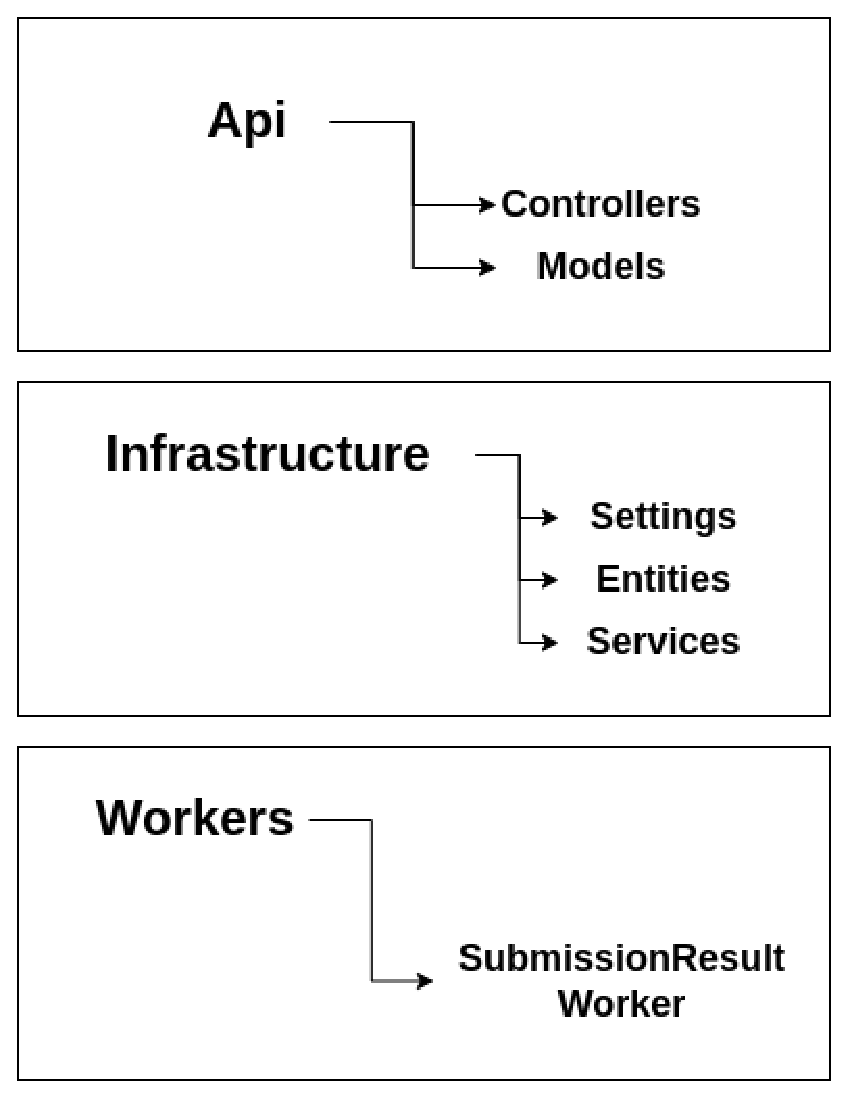
\includegraphics[keepaspectratio=true,scale=0.5]{figuras/gamma_judge_api_folders.eps}
    \caption{Esquema de pastas Gamma Judge API}
    \label{fig:judge_ui_folders}
\end{figure}

\subsubsection{Módulo de problemas}
\label{subsubsec:moduloDeProblemas}

O módulo de problemas é responsável pelos problemas e todas as funcionalidades relacionadas às informações expostas para interface da aplicação. A Figura \ref{fig:problems_endpoints} representa os endereços expostos via API pelo módulo de problemas.

\begin{figure}[H]
    \centering
    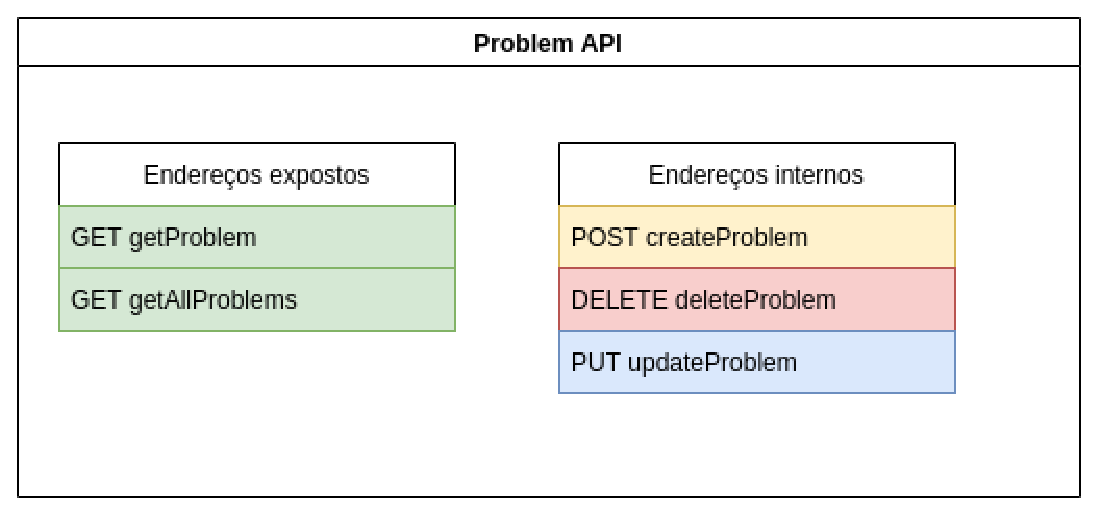
\includegraphics[keepaspectratio=true,scale=0.5]{figuras/problems_endpoins.eps}
    \caption{Funções expostas do módulo de problemas}
    \label{fig:problems_endpoints}
\end{figure}

A Figura \ref{fig:problems_endpoints} mostra em \textbf{Endereços expostos} os endereços que devem ser públicos, acessados pela interface via API; os \textbf{Endereços internos} demonstrados mostram funções da \textit{API} realizados para uso interno, possibilitando o cadastro, edição e remoção de um problema sem a necessidade da comunicação direta com o banco de dados.

\subsubsection{Módulo de eventos}
\label{subsec:moduloDeEventos}

O módulo de eventos é responsável pelas informações expostas relacionadas aos eventos cadastrados no banco de dados. A Figura \ref{fig:contests_endpoint} exemplifica o funcionamento desse módulo da API.

\begin{figure}[H]
    \centering
    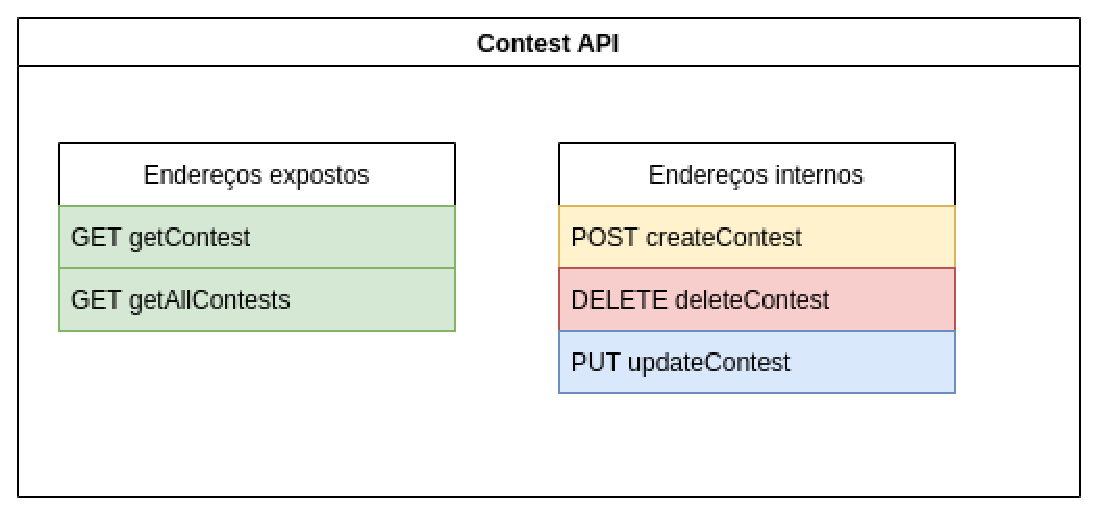
\includegraphics[keepaspectratio=true,scale=0.5]{figuras/contests_endpoint.eps}
    \caption{Funções expostas do módulo de eventos}
    \label{fig:contests_endpoint}
\end{figure}

O comportamento desse módulo é similar ao do módulo de problemas (Subseção \ref{subsubsec:moduloDeProblemas}). Ele expõe endereços internos, compostos por funções de criação, edição e remoção de eventos. Além disso, são disponibilizadas funções para recuperação de um único evento ou de vários eventos.

\subsection{Gamma Judge UI}
\label{sec:gamaJudgeUI}

A interface da aplicação é um site, com páginas que abrangem as questões e os eventos. O objetivo da interface é organizar as informações da API para o usuário, e ser uma porta de entrada para as submissões.

% A interface de usuário se concentra em um site. A aplicação tem o foco de ser simples e possuir módulos facilmente editáveis e substituíveis. Com base nisso a ferramenta de desenvolvimento da interface foi o \textit{React} \cite{rawat2020react}, utilizando \textit{Typescript} \cite{richards_et_al:CTTS} como linguagem principal.

% A ideia da interface ser dividida em componentes, visa a reutilização dos mesmos. Atualmente existem várias aplicações para juízes online, eles podem ser utilizados para o aprendizado em disciplinas de programação \cite{francisco2016juiz}, podem ser utilizados para competições de programação \cite{halim2013competitive} ou para armazenar questões de eventos, como funciona hoje no site da Olimpíada brasileira de informática \cite{obi2021}.

% Com a arquitetura e componentes divididos a interface pode ser adaptada para outras aplicações. A arquitetura em micro serviços permite futuramente que essa aplicação seja usada para outros fins de maneira mais fácil \ref{sec:microServicos}.
% TODO -- Ver o que fazer com o texto comentado 

\subsubsection{Questões}

O módulo de questões na interface é responsável por disponibilizar ao usuário as informações a respeito das questões. Os dados disponíveis aqui são referentes aos dados da Subseção \ref{subsubsec:moduloDeProblemas}. Na Figura \ref{fig:question3} é possível observar a organização e a maneira com que os dados são disponibilizados ao usuário.

\begin{figure}[H]
    \centering
    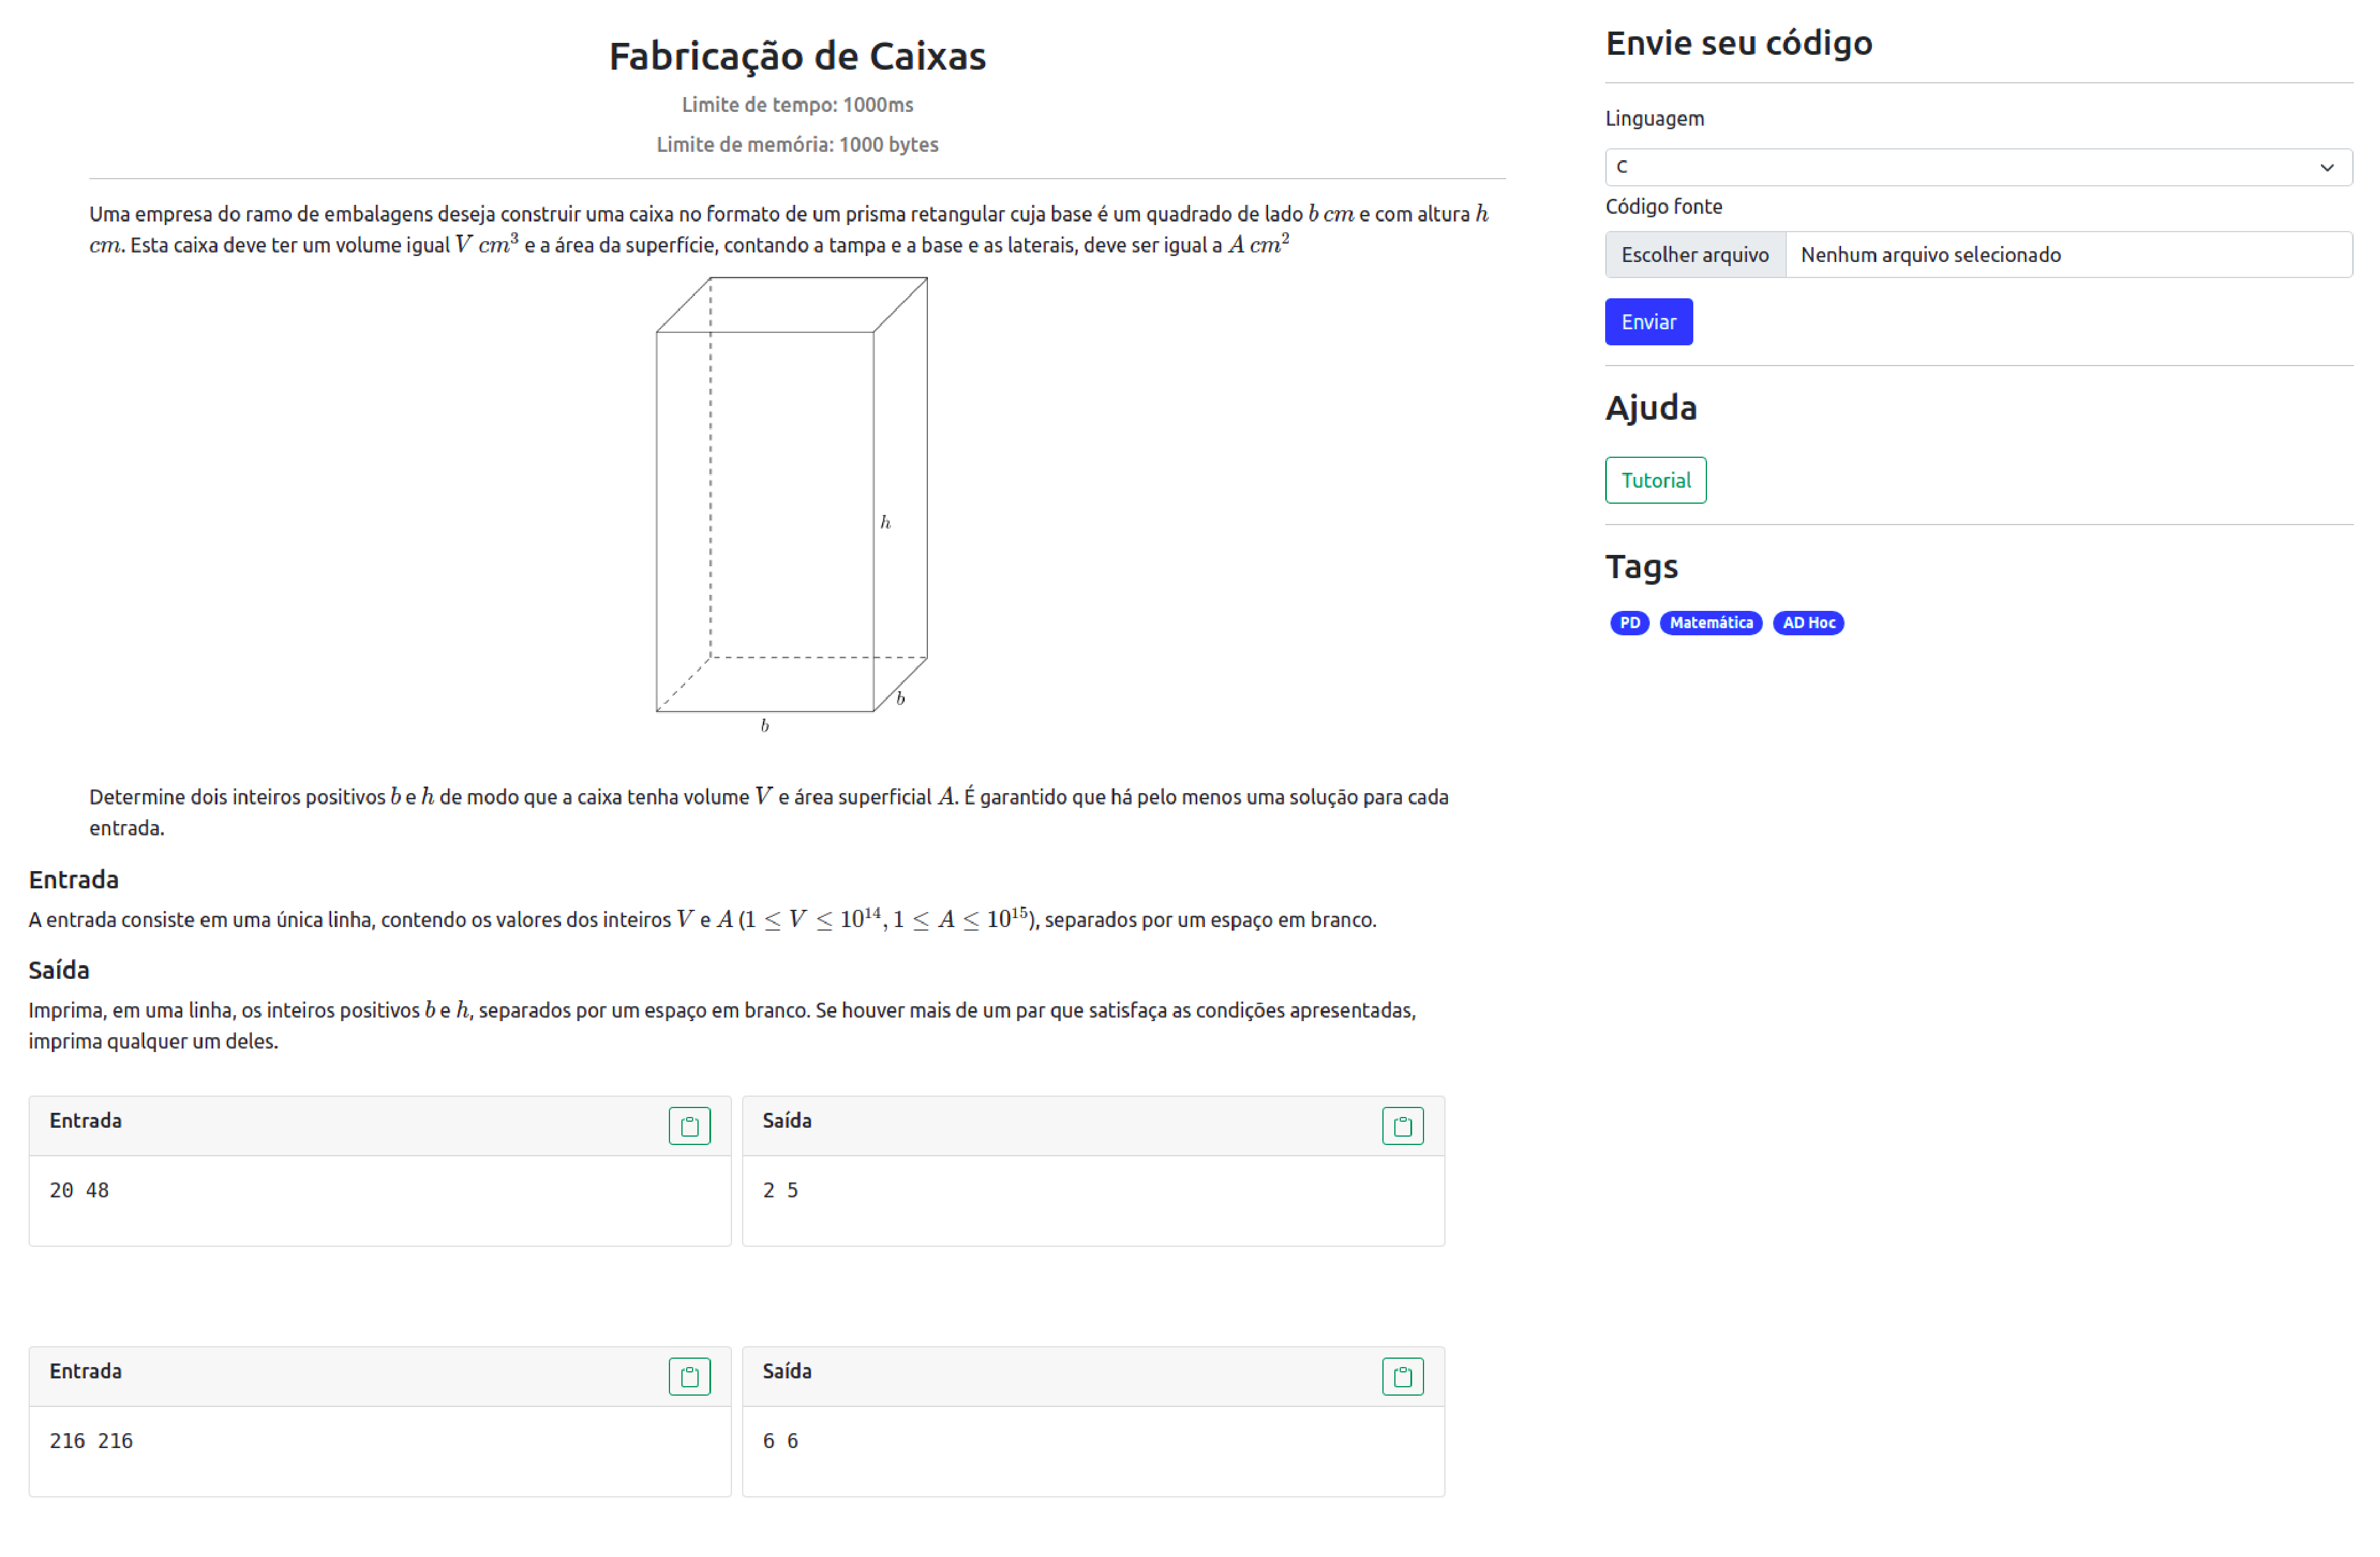
\includegraphics[keepaspectratio=true,scale=0.2]{figuras/question3.eps}
    \caption{Interface - informações da questão}
    \label{fig:question3}
\end{figure}

A interface das questões é dividida em algumas partes: o menu lateral, observável na Figura \ref{fig:sendQuestion1} no Apêndice \ref{appendix:a}; as entradas e saídas, disponíveis na Figura \ref{fig:questionInputs} no Apêndice \ref{appendix:a}; o enunciado, disponível na Figura \ref{fig:questionStatement2} no Apêndice \ref{appendix:a}.

Em juízes online elementos não textuais são bastante comuns para dar mais riquezas e detalhes às questões. Assim sendo, é comum a utilização de imagens, fórmulas matemáticas, e elementos para enfatizar trechos das questões, como textos em negrito ou itálico. Além de apresentar as informações do problema a interface também é responsável por representar elementos da API, em HTML\footnote{RAGGETT, Dave et al. HTML 4.01 Specification. W3C recommendation, v. 24, 1999.}  ou LaTEX\footnote{LAMPORT, Leslie. LaTeX. Company Cyfronet, 1991.}, em elementos não textuais; a Figura \ref{fig:questionStatement} exemplifica a utilização desses recursos.

% Para entregar flexibilidade na utilização de elementos não textuais foi utilizado o recurso NPM. A biblioteca utilizada para a visualização de elementos textuais foi o \textit{\textbf{react-latex}} \cite{reactlatex}. Essa biblioteca da flexibilidade ao usuário para utilizar elementos presentes na linguagem LaTEX e a utilização de \textit{tags} HTMLpara a inclusão de elementos não textuais como imagens.
% TODO -- Colocar na metodologia


\begin{figure}[H]
    \centering
    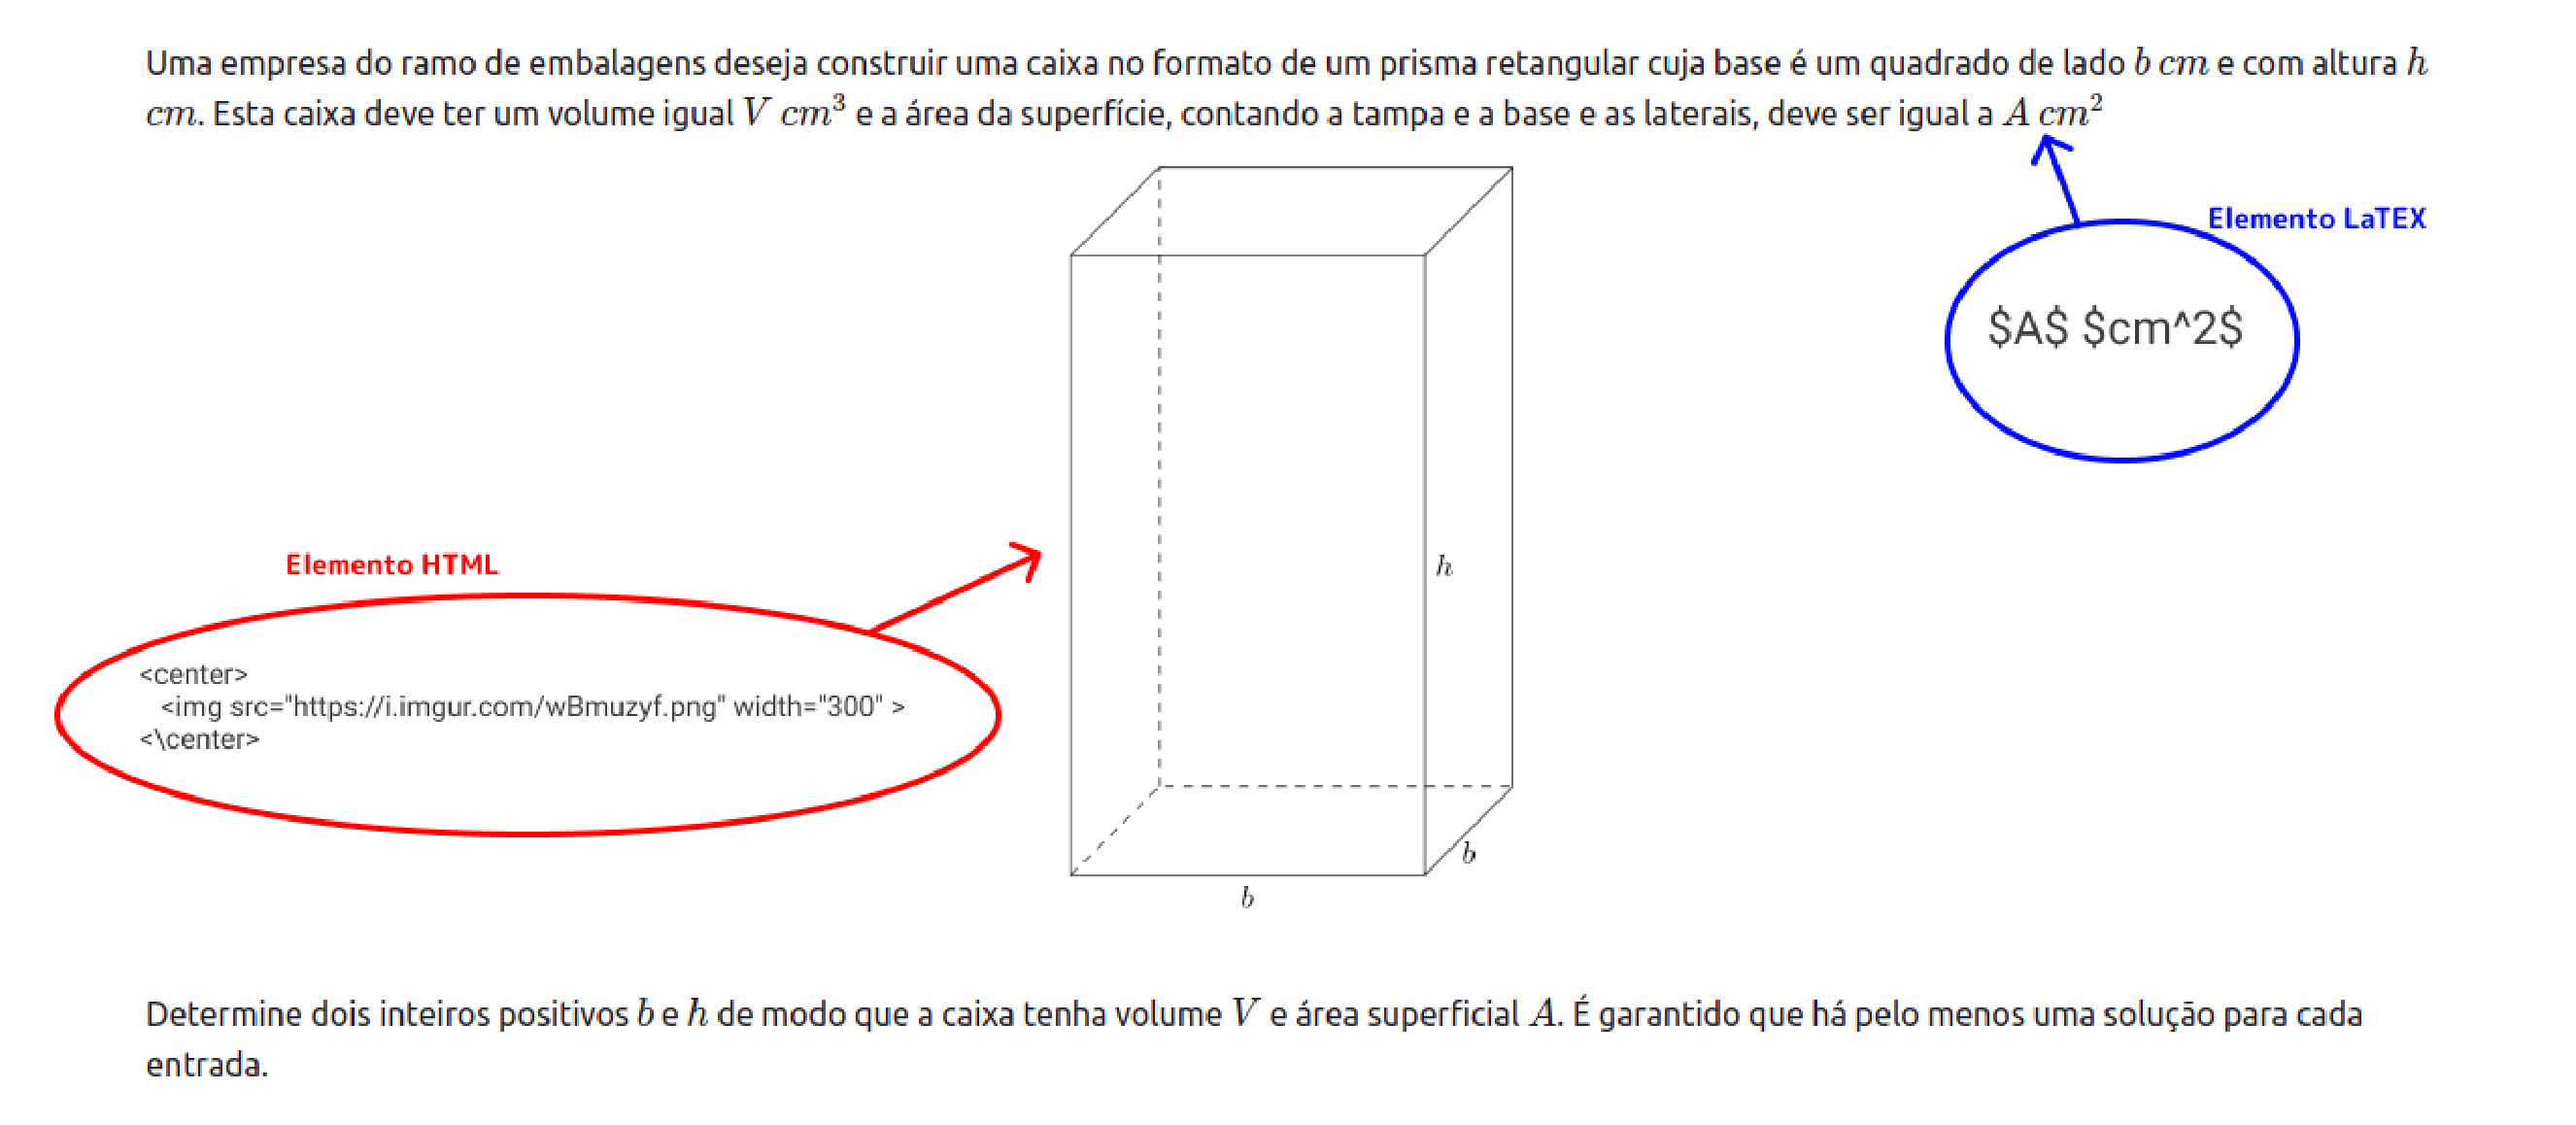
\includegraphics[keepaspectratio=true,scale=0.35]{figuras/questionStatement.eps}
    \caption{Interface — demonstração de elementos não textuais}
    \label{fig:questionStatement}
\end{figure}

A Figura \ref{fig:questionStatement} apresentada foi renderizada automaticamente a partir de um texto bruto vindo da API. O texto bruto utilizado está disponível na Figura \ref{fig:statementText} no apêndice \ref{appendix:a}, tal como o resultado da sua renderização realizada pela aplicação, disponível na Figura \ref{fig:questionStatement2} no apêndice \ref{appendix:a}. Como demostrado na Figura \ref{fig:questionStatement}, neste enunciado foi utilizado elementos da linguagem LaTEX em azul, e elementos HTML em vermelho.

\subsubsection{Eventos}
\label{subsec:eventos}

O módulo de eventos concentra as informações referentes a um determinado evento da Maratona UnB de Programação. Nesse módulo está concentrada a lista de questões do evento e a data em que ocorreu. As questões de um evento podem ser futuramente reaproveitadas em outras, portanto, também é apresentado a origem da questão, podendo ser original do evento ou podendo apresentar onde ela teve origem. A Figura \ref{fig:maratonaUnB} demostra a maneira que as informações são disponibilizadas ao usuário na tela.

\begin{figure}[H]
    \centering
    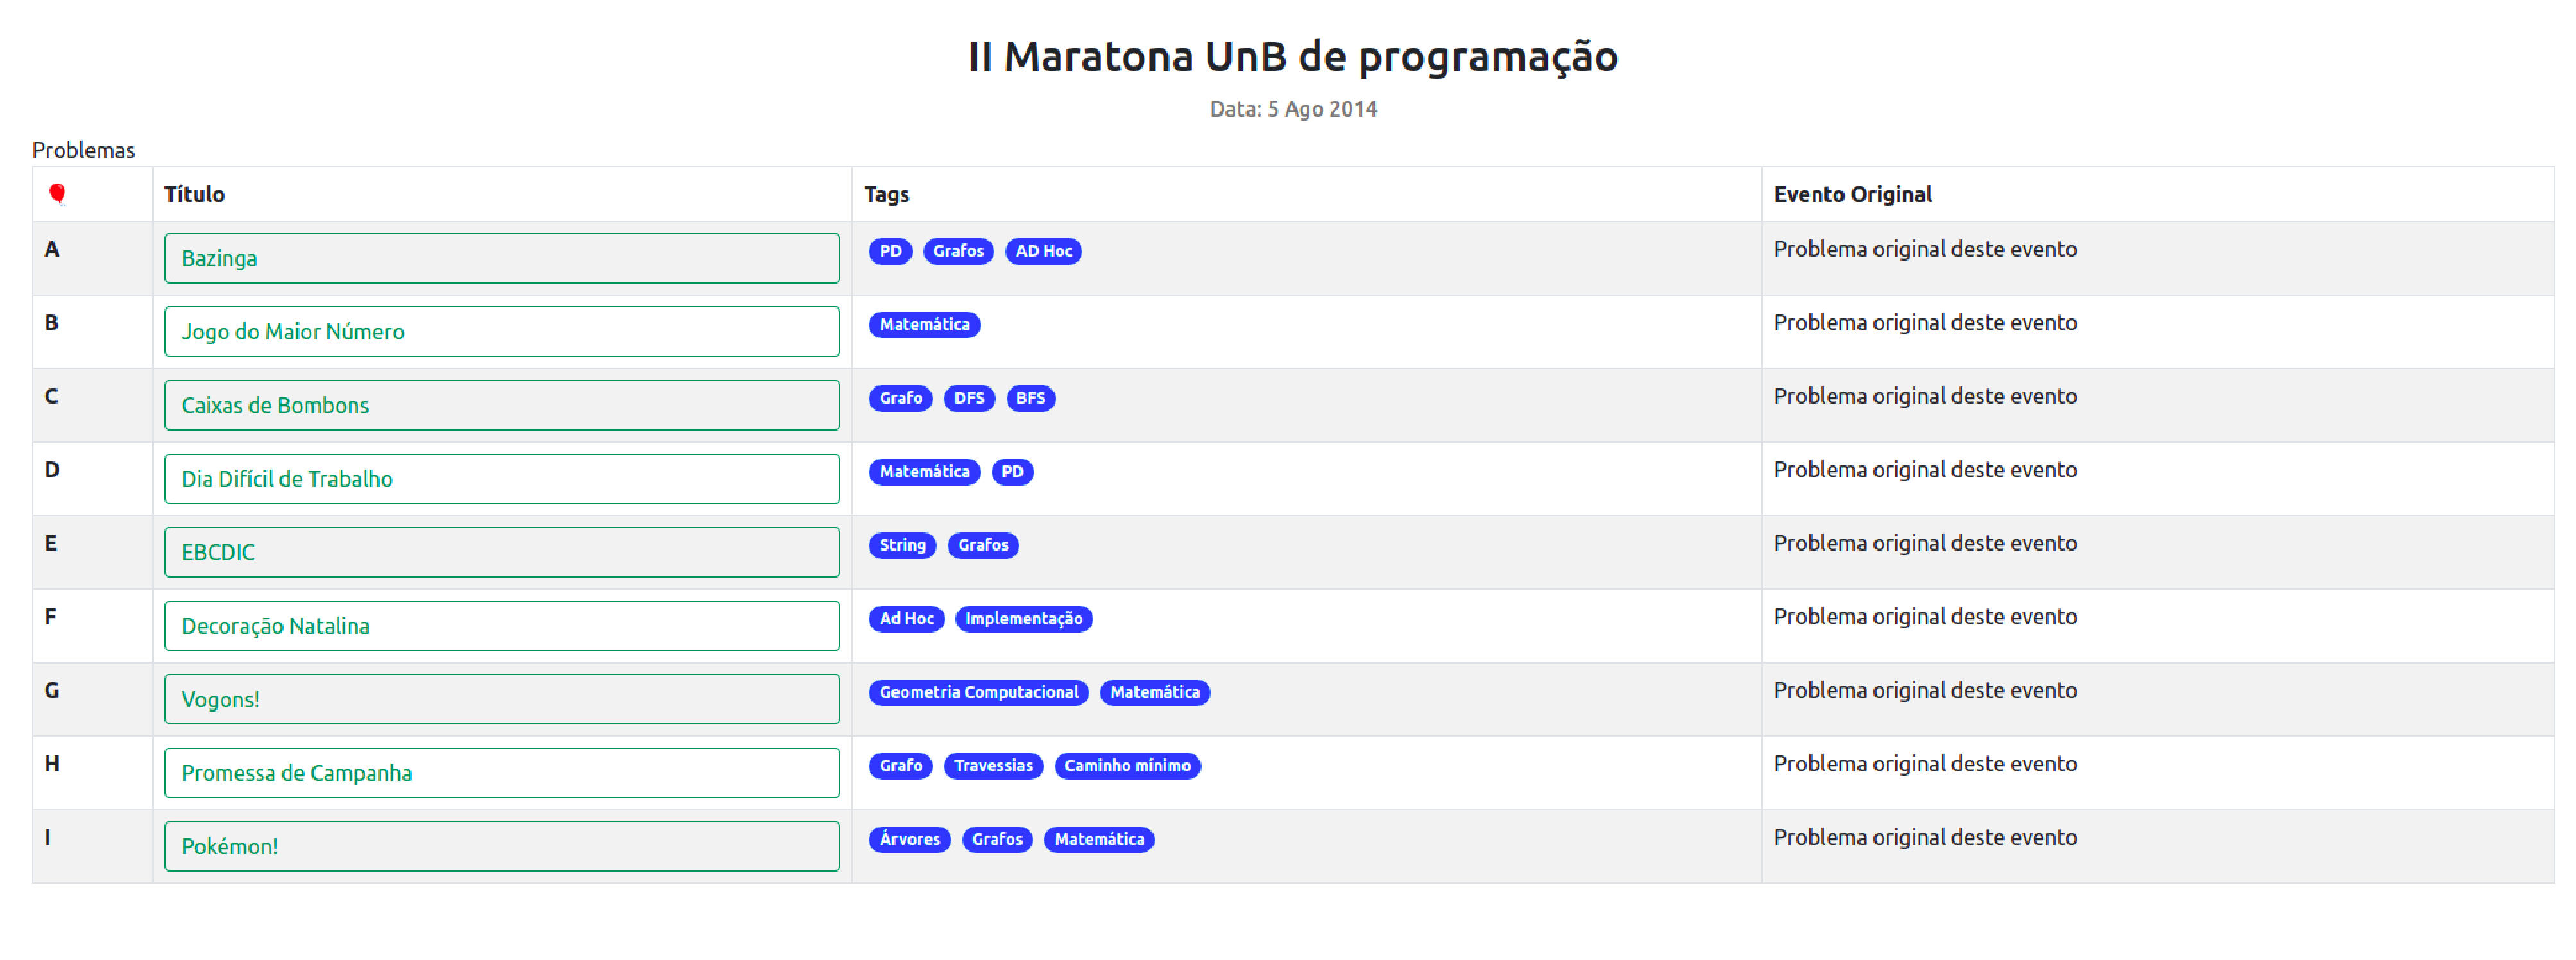
\includegraphics[keepaspectratio=true,scale=0.23]{figuras/contest2.eps}
    \caption{Interface - Detalhes de um evento}
    \label{fig:maratonaUnB}
\end{figure}


Como demonstrado na Figura \ref{fig:maratonaUnB}, são disponibilizadas informações do rótulo da questão\footnote{O rótulo é representado na Figura \ref{fig:maratonaUnB} com um ícone de balão}, título, marcações\footnote{As marcações são representadas na Figura \ref{fig:maratonaUnB} como \textit{tags}} e o evento original da questão. Diferente do que mostra a Figura \ref{fig:maratonaUnB}, é possível que nos eventos as questões sejam marcadas com rótulos diferentes das letras do alfabeto. Além disso, o campo ``Evento original'' poderia mostrar um botão para o evento em que aquele problema foi criado, caso ele tenha sido re-aproveitado nessa maratona.

\subsection{Gamma Judge Tools}
\label{sec:gamaJudgeTools}

Essa parte do sistema é responsável por julgar as submissões enviadas e retornar o veredicto, para isso foi utilizada a ferramenta de código aberto moj tools\footnote{https://github.com/cd-moj/mojtools}, responsável por executar um código e comparar as saídas com as saídas esperadas.

\begin{figure}[H]
    \centering
    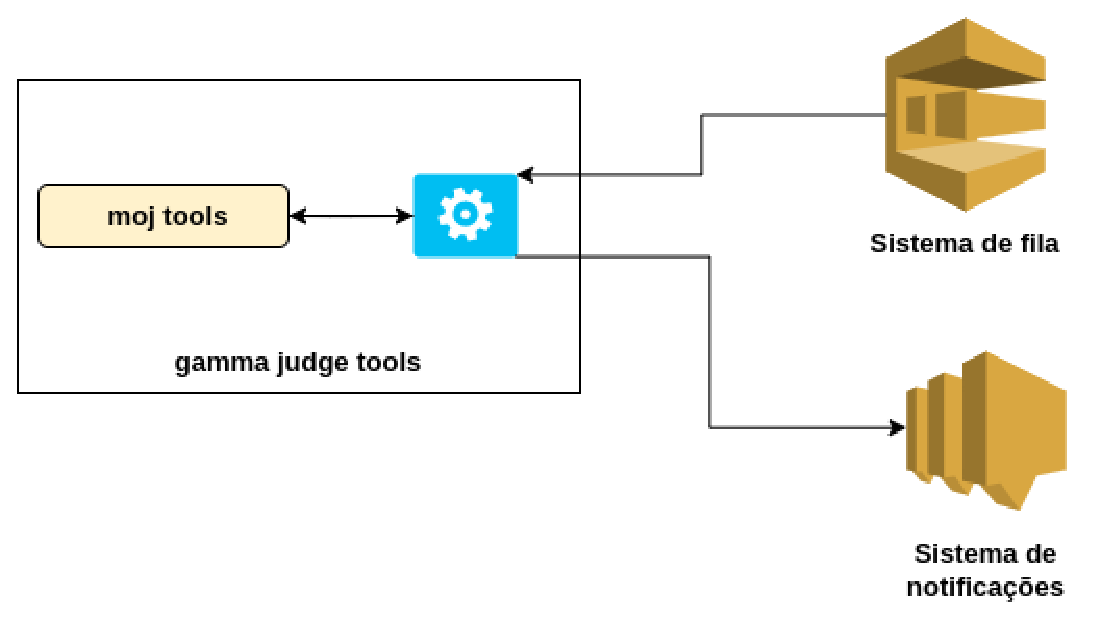
\includegraphics[keepaspectratio=true,scale=0.5]{figuras/gamma_judge_tools_diagram.eps}
    \caption{Gamma judge tools — Diagrama}
    \label{fig:judge_tools_diagram}
\end{figure}

Na Figura \ref{fig:judge_tools_diagram}, a aplicação lê do sistema de filas uma mensagem contendo as informações da submissão, após a aplicação utilizar o moj tools para julgar, o veredicto é retornado para um sistema de notificações, com isso as outras aplicações são responsáveis por lidar com a notificação enviada e processar o veredicto da submissão. 

\subsection{Gamma Judge Admin}
\label{sec:gamaJudgeAdmin}

A interface \textit{Gamma Judge Admin} auxilia o uso da API, com mecanismos para ler, criar, editar e deletar, um evento ou um problema, esse módulo não é necessário para o funcionamento da aplicação, porém, ele auxilia a manutenção e edição do conteúdo dos problemas armazenados. Sua estrutura se divide em 3 páginas:\textit{ “HomePage”}, que possui apenas botões para as outras páginas; \textit{``ProblemPage''}, que possui os mecanismos descritos, direcionados para os problemas; \textit{``ContestPage''} é como \textit{``ProblemPage''}, porém direcionada para eventos.

\subsubsection{Problem Page}

A pagina de problemas acessa a API apresentada na Subseção \ref{sec:gammaJudgeApi}, tento como base o \textit{customId}, uma sequência de caracteres que identifica cada um dos problemas unicamente. A Figura \ref{fig:judge_admin_problem} representa a página descrita; com o botão \textit{``GET''}, em verde, e o \textit{customId} preenchido, é possível recuperar as informações de um problema; \textit{``PUT''}, em azul, cria, caso o  não exista, ou sobrescreve as informações do problema; \textit{``DELETE''}, em vermelho, apaga o problema.

\begin{figure}[H]
    \centering
    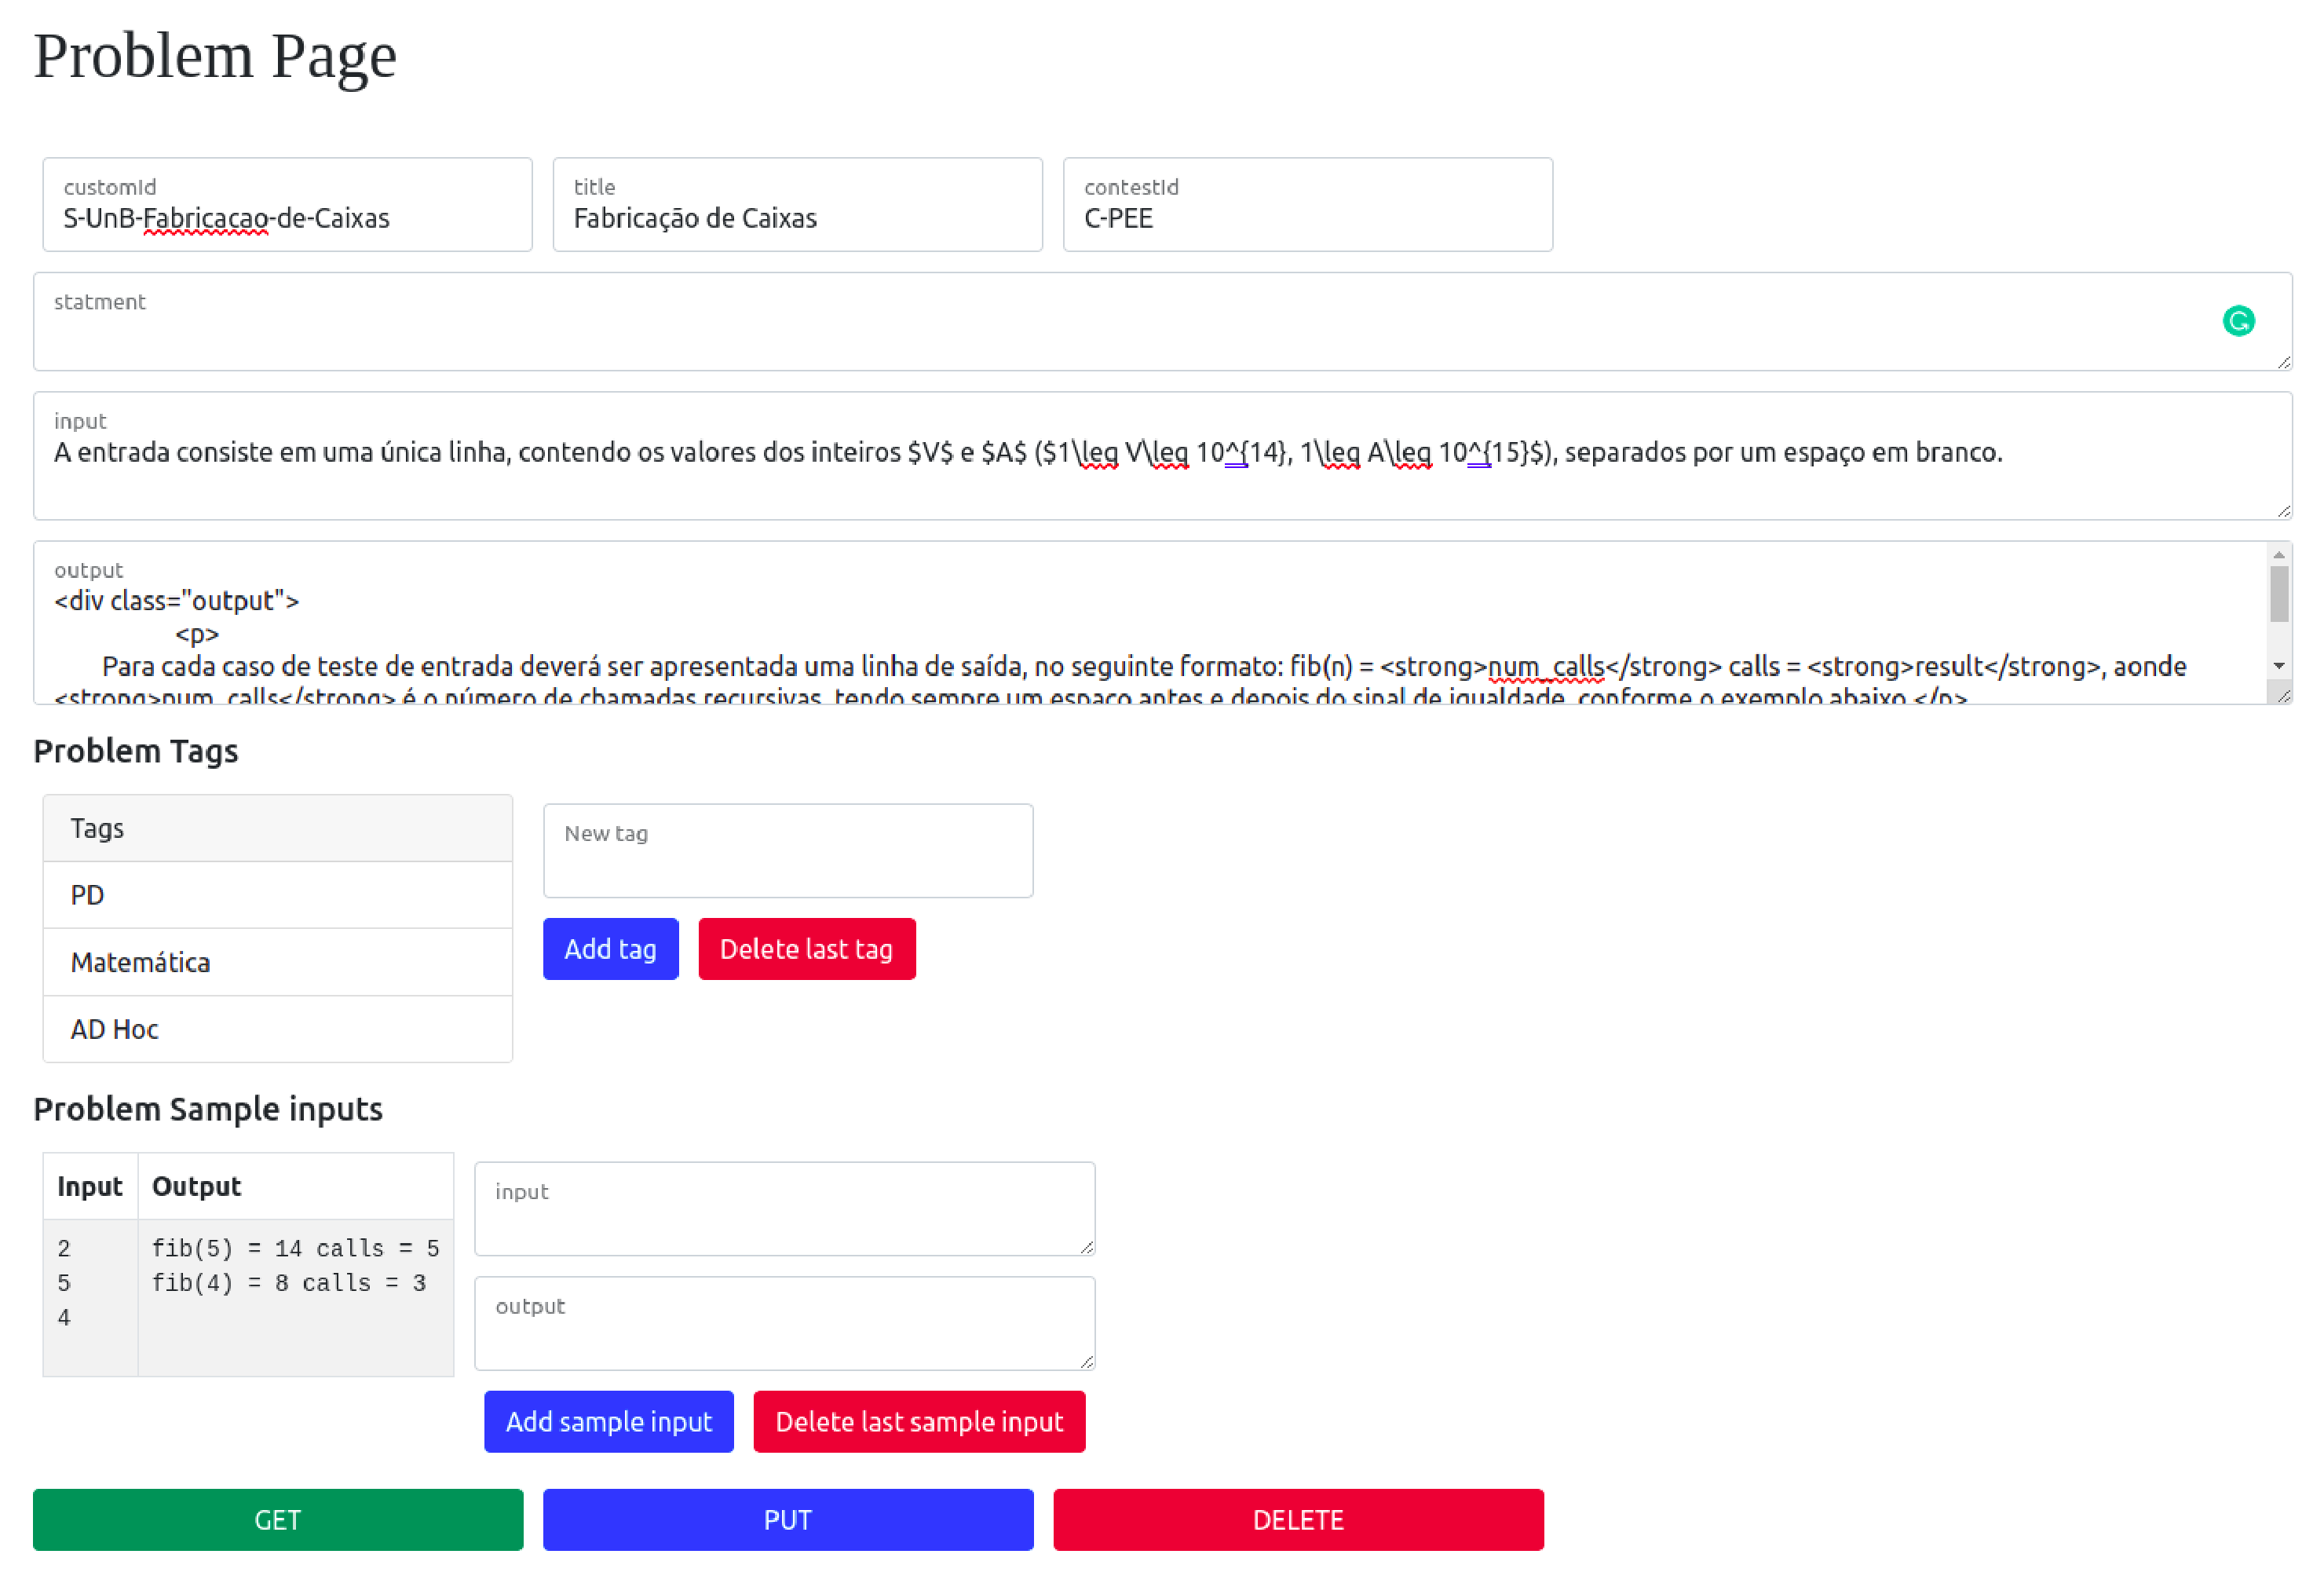
\includegraphics[keepaspectratio=true,scale=0.32]{figuras/problem_page.eps}
    \caption{Gamma judge Admin — ProblemPage}
    \label{fig:judge_admin_problem}
\end{figure}

\subsubsection{Contest Page}

A página de eventos tem o comportamento similar a página de problemas, com os mesmos botões e mesmo funcionamento, porém com menos informações. Na página de eventos é possível adicionar ou remover problemas ao evento utilizando o \textit{customId} do problema e o \textit{identifier}, será o identificador do problema naquele evento, como mostra na Figura \ref{fig:judge_admin_contest}.

\begin{figure}[H]
    \centering
    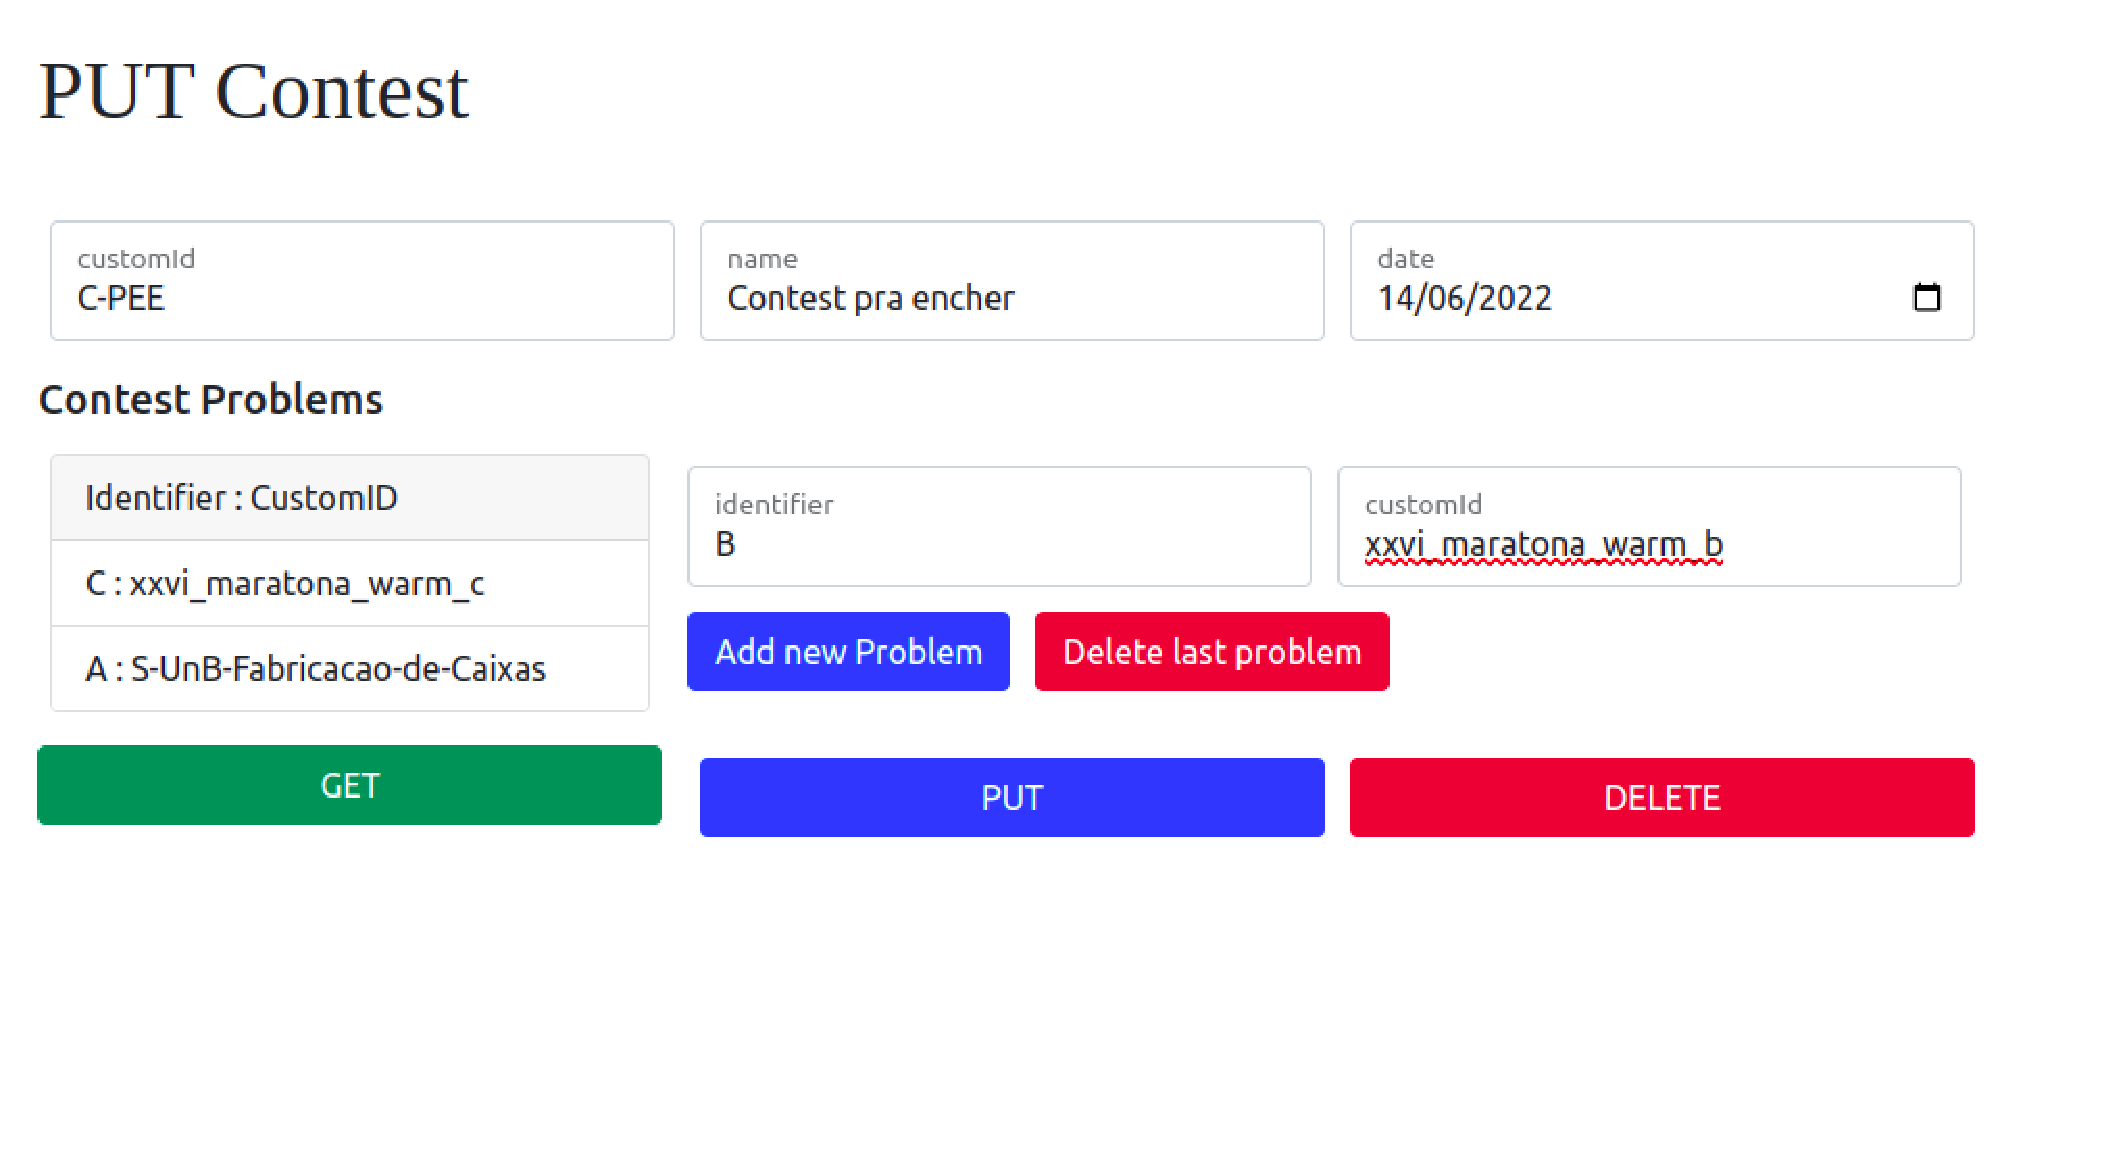
\includegraphics[keepaspectratio=true,scale=0.45]{figuras/contest_page.eps}
    \caption{Gamma judge Admin — ContestPage}
    \label{fig:judge_admin_contest}
\end{figure}

\bookmarksetup{startatroot}

\postextual

\bibliography{bibliografia}
\begin{anexosenv}

    \partanexos

    \chapter{Primeiro Anexo}

    Texto do primeiro anexo.

    \chapter{Segundo Anexo}

    Texto do segundo anexo.

\end{anexosenv}


\begin{apendicesenv}

    \partapendices

    \chapter{Primeiro Apêndice}

    Texto do primeiro apêndice.

    \chapter{Segundo Apêndice}

    Texto do segundo apêndice.

\end{apendicesenv}

\printindex

\end{document}

